%----------------------------------------------------------------------------------------
%	PACKAGES AND THEMES
%----------------------------------------------------------------------------------------


\documentclass{beamer}

\mode<presentation> {

% The Beamer class comes with a number of default slide themes
% which change the colors and layouts of slides. Below this is a list
% of all the themes, uncomment each in turn to see what they look like.


\usepackage{qtree}
%\usetheme{default}
%\usetheme{AnnArbor}
%\usetheme{Antibes}
%\usetheme{Bergen}
%\usetheme{Berkeley}
%\usetheme{Berlin}
%\usetheme{Boadilla}
%\usetheme{CambridgeUS}
%\usetheme{Copenhagen}
%\usetheme{Darmstadt}
%\usetheme{Dresden}
%\usetheme{Frankfurt}
%\usetheme{Goettingen}
%\usetheme{Hannover}
%\usetheme{Ilmenau}
%\usetheme{JuanLesPins}
%\usetheme{Luebeck}
\usetheme{Madrid}
%\usetheme{Malmoe}
%\usetheme{Marburg}
%\usetheme{Montpellier}
%\usetheme{PaloAlto}
%\usetheme{Pittsburgh}
%\usetheme{Rochester}
%\usetheme{Singapore}
%\usetheme{Szeged}
%\usetheme{Warsaw}

% As well as themes, the Beamer class has a number of color themes
% for any slide theme. Uncomment each of these in turn to see how it
% changes the colors of your current slide theme.

%\usecolortheme{albatross}
%\usecolortheme{beaver}
%\usecolortheme{beetle}
%\usecolortheme{crane}
%\usecolortheme{dolphin}
%\usecolortheme{dove}
%\usecolortheme{fly}
%\usecolortheme{lily}
%\usecolortheme{orchid}
%\usecolortheme{rose}
%\usecolortheme{seagull}
%\usecolortheme{seahorse}
%\usecolortheme{whale}
%\usecolortheme{wolverine}

%\setbeamertemplate{footline} % To remove the footer line in all slides uncomment this line
%\setbeamertemplate{footline}[page number] % To replace the footer line in all slides with a simple slide count uncomment this line

%\setbeamertemplate{navigation symbols}{} % To remove the navigation symbols from the bottom of all slides uncomment this line
}

\usepackage{graphicx} % Allows including images
\usepackage{booktabs} % Allows the use of \toprule, \midrule and \bottomrule in tables

%----------------------------------------------------------------------------------------
%	TITLE PAGE
%----------------------------------------------------------------------------------------

\title[Wavelet Tree]{Engineering Rank and Select Queries on Wavelet Trees} % The short title appears at the bottom of every slide, the full title is only on the title page

\author{Roland Larsen Pedersen} % Your name
\institute[Datalogi] % Your institution as it will appear on the bottom of every slide, may be shorthand to save space
{
Datalogi, Aarhus Universitet \\ % Your institution for the title page
\medskip
\textit{Thesis defence}
}
\date{June 25, 2015} % Date, can be changed to a custom date

\begin{document}

\begin{frame}
\titlepage % Print the title page as the first slide
\end{frame}

\begin{frame}
\frametitle{Overview} % Table of contents slide, comment this block out to remove it
\tableofcontents % Throughout your presentation, if you choose to use \section{} and \subsection{} commands, these will automatically be printed on this slide as an overview of your presentation
\end{frame}

%----------------------------------------------------------------------------------------
%	PRESENTATION SLIDES
%----------------------------------------------------------------------------------------


\section{What is a Wavelet Tree?}

\subsection{Definitions}
\begin{frame}
\frametitle{Wavelet Tree: Definitions}
\begin{itemize}
\item In its basic form, the wavelet tree is a balanced binary tree. 
\item It stores a \textit{sequence} $S[1,n] = c_1c_2c_3 \ldots c_n$ of \textit{symbols} $c_i \in \Sigma$, where $\Sigma = [1 \ldots \sigma]$ is the \textit{alphabet} of $S$.
\item The tree has height $h = \lceil \log \sigma \rceil$, and $2 \sigma - 1$ nodes, with $\sigma$ of those as leaf nodes and $\sigma - 1$ as internal nodes.
\end{itemize}

\end{frame}


%------------------------------------------------

\begin{frame}
\frametitle{Constructing the Wavelet Tree}
\begin{itemize}
\item The wavelet tree is constructed recursively, starting at the root node and moving down the tree, with each node in the tree receiving a string constructed by its parent, except the root node that receives the full input string.
\item Each node calculates the middle character of $\Sigma$ and uses it to set the bits in the bitmap and split $S$ in two substrings $S_{\mathit{left}}$ and $S_{\mathit{right}}$.
\end{itemize}
\end{frame}

%------------------------------------------------
\subsection{Constructing the Wavelet Tree}
\begin{frame}
\frametitle{Wavelet Tree Example}
\Tree
%root
[.adsfadaadsfaads\\001100000110001 !\qsetw{5cm} 
	%left child
	[.adadaadaad\\0101001001 !\qsetw{5cm}
		%left -> left,right child 
		[.aaaaaa !\qsetw{5cm} ] [.dddd !\qsetw{5cm} ]] 
	%right child
	[.sfsfs\\10101 !\qsetw{5cm} 
		%right -> left,right child
		[.ff !\qsetw{5.3cm} ] [.sss !\qsetw{5.3cm} ]]] 
\vspace*{1cm}		
$S = \text{adsfadaadsfaads}, \Sigma = \text{adfs}$
\end{frame}

%------------------------------------------------
\begin{frame}
\frametitle{Construction time and memory usage}
\begin{itemize}
\item Construction time: $O(n \cdot h) = O(n \log \sigma)$
	\begin{itemize}
	\item The Wavelet Tree can theoretically be constructed in $O(n \cdot h) = O(n \log \sigma)$ time as the sum of the lengths of the strings being processed at any single layer of the tree is the length of the input string to the tree.
	\end{itemize}
\item Memory usage: $O(n \log \sigma + \sigma \cdot \mathit{ws})$ bits
	\begin{itemize}
	\item At each level in the tree at most \textit{n} bits are stored in the bitmaps in total, making $n \cdot h = n \cdot \log \sigma$ an upper bound to the total number of bits that a wavelet tree stores in its bitmaps.
\item In addition to this, each node takes some constant amount of machine words of space, and there are $2 \sigma -1$ nodes in the tree.
\textit{ws} is the size of our machine words.
This makes the total memory consumption $O(n \log \sigma + \sigma \cdot \mathit{ws})$ bits.
	\end{itemize}
\end{itemize}
\end{frame}

\section{Queries}
%------------------------------------------------
\begin{frame}
\frametitle{Wavelet Tree: Queries}
\begin{itemize}
\item The wavelet tree supports three queries:
	\begin{itemize}
	\item \textbf{Access(p)}: Return the character \textit{c} at position \textit{p} in sequence \textit{S}.
	\item \textbf{Rank(c, p)}: Return the number of occurrences of character \textit{c} in \textit{S} up to position \textit{p}.
		\begin{itemize}
		\item Running time: $O(n \log \sigma)$
		\end{itemize}
	\item \textbf{Select(c, o)}: Return the position of the \textit{o}th occurrence of character \textit{c} in \textit{S}.
		\begin{itemize}
		\item Running time: $O(n \log \sigma)$
		\end{itemize}
		\end{itemize}
\end{itemize}

\end{frame}

%------------------------------------------------

\subsection{Rank}
\begin{frame}
\frametitle{Rank on a Wavelet Tree}
\begin{center}
	\center 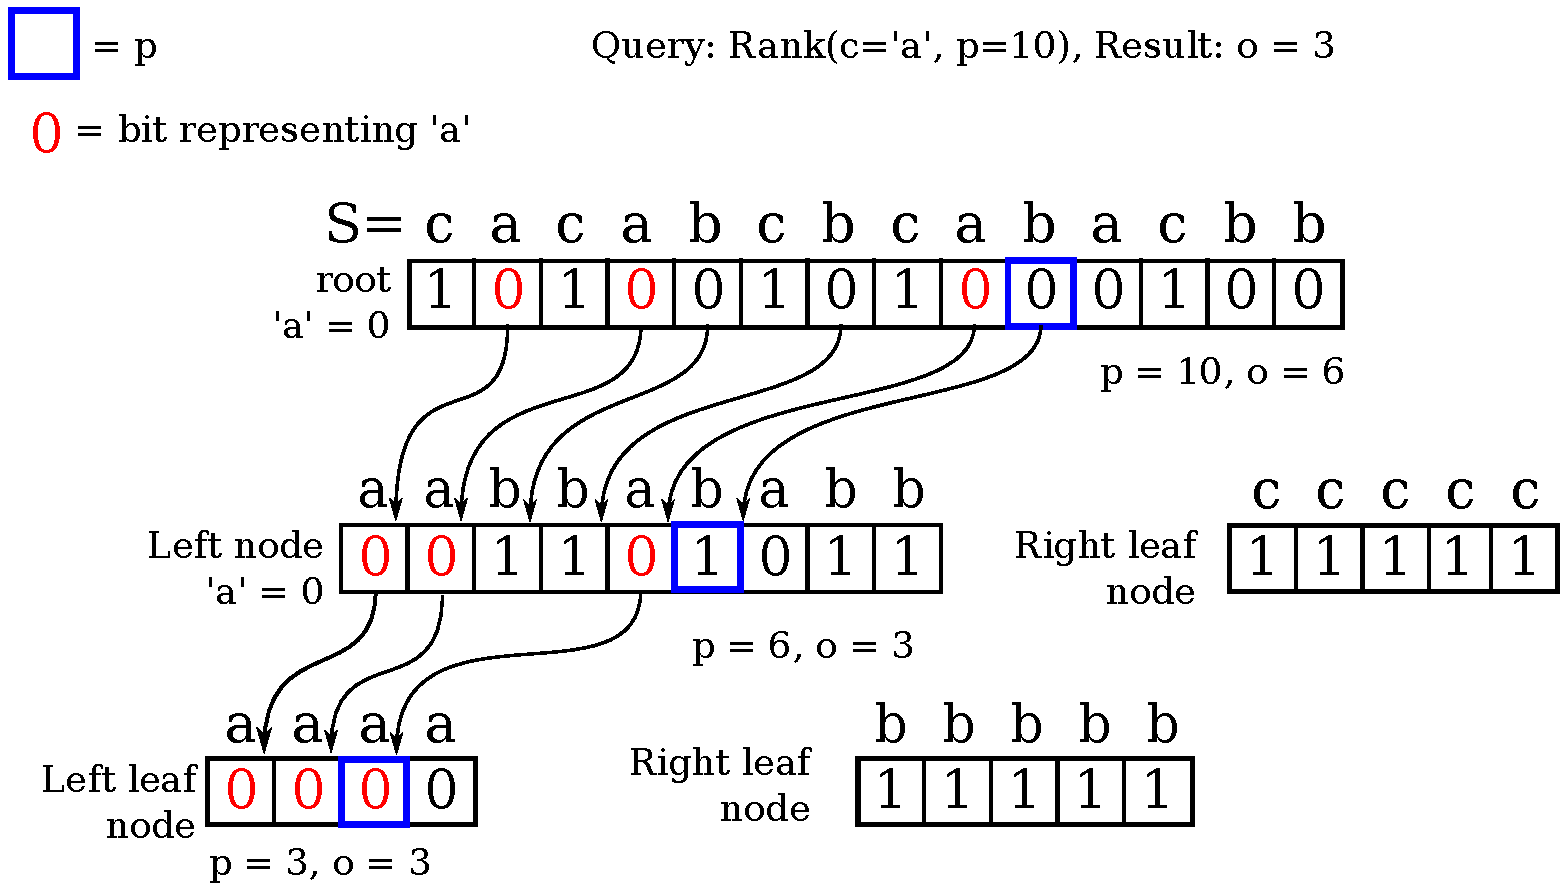
\includegraphics[width=0.8\textwidth]{RankDrawing}
\end{center}
\end{frame}

\subsection{Select}
\begin{frame}
\frametitle{Select on a Wavelet Tree}
\begin{center}
	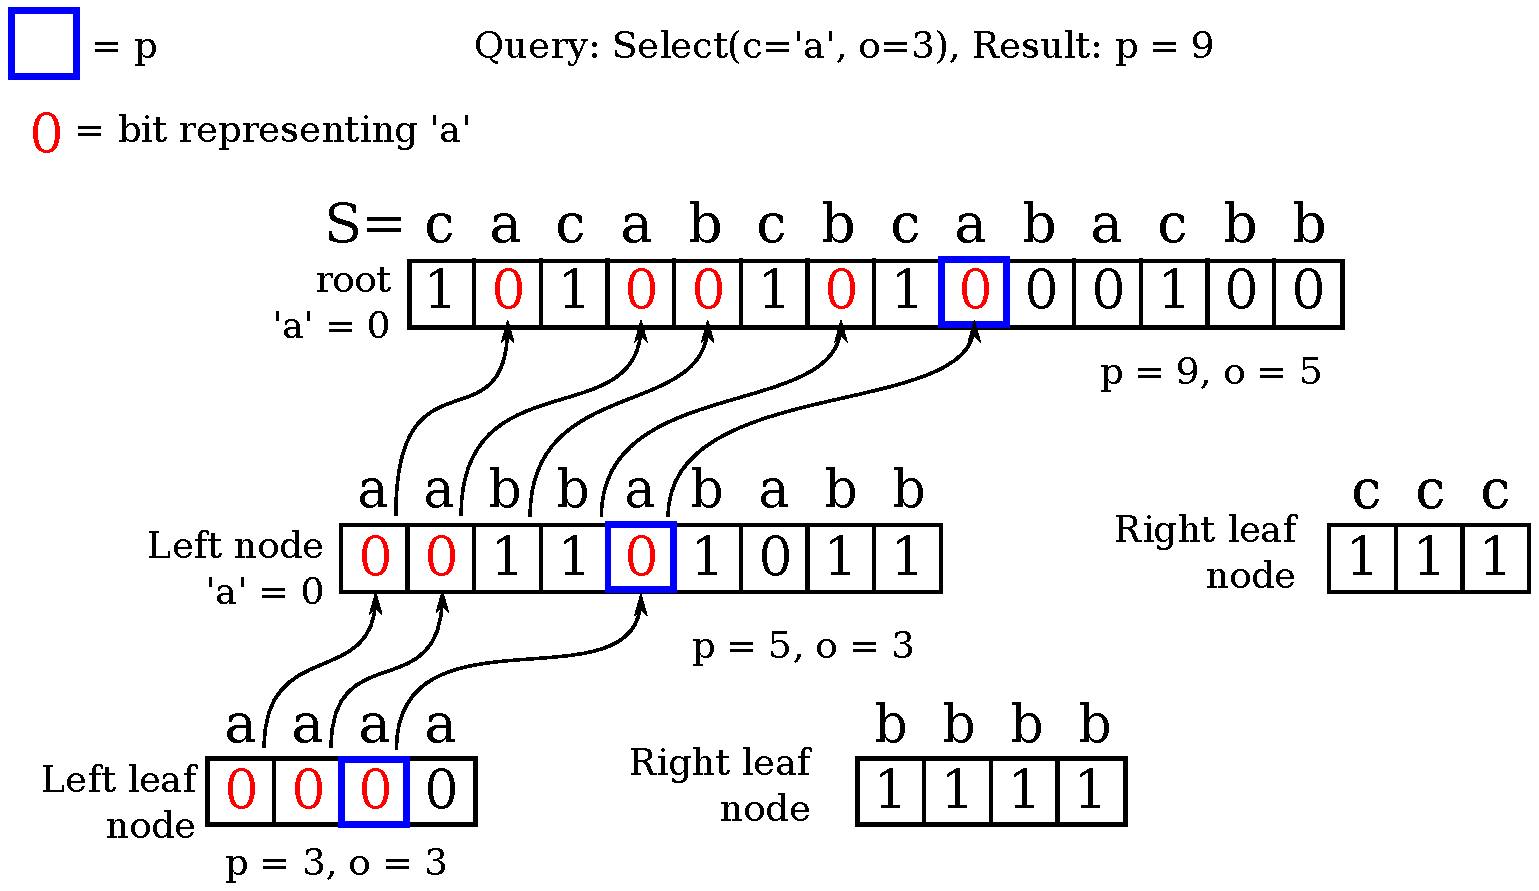
\includegraphics[width=0.8\textwidth]{SelectDrawing}
\end{center}
\end{frame}

\begin{frame}
\frametitle{Blocks of Highlighted Text}
\begin{block}{Block 1}
Lorem ipsum dolor sit amet, consectetur adipiscing elit. Integer lectus nisl, ultricies in feugiat rutrum, porttitor sit amet augue. Aliquam ut tortor mauris. Sed volutpat ante purus, quis accumsan dolor.
\end{block}

\begin{block}{Block 2}
Pellentesque sed tellus purus. Class aptent taciti sociosqu ad litora torquent per conubia nostra, per inceptos himenaeos. Vestibulum quis magna at risus dictum tempor eu vitae velit.
\end{block}

\begin{block}{Block 3}
Suspendisse tincidunt sagittis gravida. Curabitur condimentum, enim sed venenatis rutrum, ipsum neque consectetur orci, sed blandit justo nisi ac lacus.
\end{block}
\end{frame}

%------------------------------------------------

\begin{frame}
\frametitle{Multiple Columns}
\begin{columns}[c] % The "c" option specifies centered vertical alignment while the "t" option is used for top vertical alignment

\column{.45\textwidth} % Left column and width
\textbf{Heading}
\begin{enumerate}
\item Statement
\item Explanation
\item Example
\end{enumerate}

\column{.5\textwidth} % Right column and width
Lorem ipsum dolor sit amet, consectetur adipiscing elit. Integer lectus nisl, ultricies in feugiat rutrum, porttitor sit amet augue. Aliquam ut tortor mauris. Sed volutpat ante purus, quis accumsan dolor.

\end{columns}
\end{frame}


\begin{frame}
\frametitle{Table}
\begin{table}
\begin{tabular}{l l l}
\toprule
\textbf{Treatments} & \textbf{Response 1} & \textbf{Response 2}\\
\midrule
Treatment 1 & 0.0003262 & 0.562 \\
Treatment 2 & 0.0015681 & 0.910 \\
Treatment 3 & 0.0009271 & 0.296 \\
\bottomrule
\end{tabular}
\caption{Table caption}
\end{table}
\end{frame}

%------------------------------------------------

\begin{frame}
\frametitle{Theorem}
\begin{theorem}[Mass--energy equivalence]
$E = mc^2$
\end{theorem}
\end{frame}

%------------------------------------------------

\begin{frame}[fragile] % Need to use the fragile option when verbatim is used in the slide
\frametitle{Verbatim}
\begin{example}[Theorem Slide Code]
\begin{verbatim}
\begin{frame}
\frametitle{Theorem}
\begin{theorem}[Mass--energy equivalence]
$E = mc^2$
\end{theorem}
\end{frame}\end{verbatim}
\end{example}
\end{frame}

%------------------------------------------------

\begin{frame}
\frametitle{Figure}
Uncomment the code on this slide to include your own image from the same directory as the template .TeX file.
%\begin{figure}
%\includegraphics[width=0.8\linewidth]{test}
%\end{figure}
\end{frame}

%------------------------------------------------

\begin{frame}[fragile] % Need to use the fragile option when verbatim is used in the slide
\frametitle{Citation}
An example of the \verb|\cite| command to cite within the presentation:\\~

This statement requires citation \cite{p1}.
\end{frame}

%------------------------------------------------

\begin{frame}
\frametitle{References}
\footnotesize{
\begin{thebibliography}{99} % Beamer does not support BibTeX so references must be inserted manually as below
\bibitem[Smith, 2012]{p1} John Smith (2012)
\newblock Title of the publication
\newblock \emph{Journal Name} 12(3), 45 -- 678.
\end{thebibliography}
}
\end{frame}

%------------------------------------------------

\begin{frame}
\Huge{\centerline{The End}}
\end{frame}

%----------------------------------------------------------------------------------------

\end{document} 